
\documentclass[11pt,a4paper,oneside]{report}

\usepackage[T1]{fontenc}
\usepackage[utf8]{inputenc}
\usepackage{lmodern}
\usepackage[margin=1in,headheight=15pt]{geometry}
\usepackage{microtype}
\usepackage{enumitem}
\usepackage{array,booktabs,tabularx,longtable}
\usepackage{xcolor}
\usepackage{graphicx}
\usepackage{amsmath}
\usepackage{fancyhdr}
\usepackage{xurl}
\usepackage[hidelinks]{hyperref}

\hypersetup{
  pdftitle={Distributed Load-Testing Platform: Project Report},
  pdfauthor={Jatin Bajaj and Project Team},
  pdfsubject={Software Engineering Project}
}

\urlstyle{tt}
\setlength{\parindent}{0pt}
\setlength{\parskip}{0.45em}
\setlength{\emergencystretch}{3em}
\renewcommand{\arraystretch}{1.18}

\setlist[itemize]{leftmargin=1.5em,itemsep=0.2em,topsep=0.3em}
\setlist[enumerate]{leftmargin=1.8em,itemsep=0.25em,topsep=0.3em}

\newcolumntype{Y}{>{\raggedright\arraybackslash}X}
\newcolumntype{P}[1]{>{\raggedright\arraybackslash}p{#1}}
\newcommand{\code}[1]{\texttt{\detokenize{#1}}}
\newcommand{\ReportDate}{12 October 2026}
\newcommand{\Advisor}{Dr. Paramveer Kaur}

\pagestyle{fancy}
\fancyhf{}
\fancyhead[L]{\small Distributed Load-Testing Platform}
\fancyhead[R]{\small Project Report}
\fancyfoot[C]{\thepage}
\renewcommand{\headrulewidth}{0.4pt}

\fancypagestyle{plain}{
  \fancyhf{}
  \fancyfoot[C]{\thepage}
  \renewcommand{\headrulewidth}{0pt}
}

\begin{document}

% ================================================================
% TITLE PAGE
% ================================================================

\hypersetup{pageanchor=false}

\begin{titlepage}
  \centering

  {\large\bfseries Thapar Institute of Engineering and Technology\par}
  \vspace{0.2cm}
  {\large Patiala, Punjab\par}

  \vspace{0.9cm}
  {\large Software Engineering Project\par}

  \vspace{1.1cm}
  {\Huge\bfseries Distributed Load-Testing Platform\par}

  \vspace{0.4cm}
  {\LARGE A Cloud-Assisted Load-Testing System for Local Applications\par}

  \vspace{0.8cm}
  {\Large\bfseries Prototype-Stage Project Report\par}

  \vspace{0.2cm}
  {\large Mid-Semester Progress Report\par}

  \vspace{1.2cm}
  {\large Submitted to\par}
  \vspace{0.15cm}
  {\Large\bfseries \Advisor\par}

  \vspace{1.0cm}
  {\large Submitted by\par}
  \vspace{0.3cm}

  \begin{tabular}{@{}ll@{}}
    \textbf{Student} & \textbf{Roll Number} \\
    \midrule
    Jatin Bajaj &   \texttt{   1024170389}\\
    Krish Shani &  \texttt{    1024170390} \\
    Rishabh Dutt&   \texttt{    1024170393}
  \end{tabular}

  \vfill

  {\large\bfseries Computer Science and Engineering Department\par}
  \vspace{0.4cm}
  {\large \ReportDate\par}

\end{titlepage}

\pagenumbering{roman}
\hypersetup{pageanchor=true}

% ================================================================
% ABSTRACT
% ================================================================

\chapter*{Abstract}
\addcontentsline{toc}{chapter}{Abstract}

This project aims to develop a distributed load-testing platform
that enables students and developers to evaluate applications
running on their own machines. A lightweight local agent connects
a locally hosted application to a cloud-side gateway and load
generator. The cloud component can then send test traffic through
the tunnel without requiring the student's application to be
directly exposed to the public internet.

The current prototype uses Java 21, Maven, Netty, and JavaFX.
The load-test API has been exercised locally through Postman. A
10,000-request workload has been configured and submitted in the
local environment, and the test lifecycle can be inspected through
its status endpoint. Separate completed-run evidence records 100
successful requests, zero failed requests, and response-time and
throughput metrics. These observations demonstrate local workflow
progress; the 100-request result must not be interpreted as the
result of the 10,000-request run.

The Netty gateway has been started on port 9090, and the initial
agent registration protocol has been verified. Cloud-side load
validation, broader system improvements, performance graphs, and
the frontend component remain outstanding. Complete bidirectional
HTTP forwarding through the tunnel must also be validated end to end.

This report documents the project objectives, architecture,
technology choices, implementation progress, testing status,
limitations, and next development milestones. It distinguishes
verified implementation progress from planned capabilities.

\tableofcontents
\clearpage
\pagenumbering{arabic}

% ================================================================
\chapter{Introduction}
% ================================================================

\section{Background and Context}

Load testing is used to evaluate how an application behaves when
it receives many requests over a period of time. Developers
commonly measure response time, throughput, error rate, and the
effect of concurrent requests before deploying an application.

Traditional load-testing tools can generate substantial traffic,
but distributed load generation and testing an application that
is available only on a developer's local machine can be
inconvenient.

The proposed platform focuses on this local-development scenario.
A student runs an application on \code{localhost} and starts a
lightweight local agent. The agent establishes an outbound
connection to a cloud gateway. A cloud-side load generator can
then use the tunnel to send requests to the local application.

The intended workflow is to configure a test, execute it through
the platform, and inspect the resulting performance metrics
without manually exposing the local application to the public
internet.

\section{Problem Statement}

The project addresses the following problems:

\begin{enumerate}
  \item \textbf{Local reachability:}
  A cloud worker cannot normally reach a service bound only to
  a student's local machine.

  \item \textbf{Load generation:}
  Developers need a repeatable way to configure request volume
  and concurrency.

  \item \textbf{Traffic forwarding:}
  Requests must be forwarded through a tunnel with correct
  request and response handling.

  \item \textbf{Performance measurement:}
  Test results must report meaningful metrics rather than
  merely confirming that requests were sent.

  \item \textbf{Distributed execution:}
  The design should support future load generation through
  multiple cloud workers.
\end{enumerate}

The central engineering challenge is to integrate the tunnel
and load generator while minimising additional overhead
introduced by the proxy layer. The initial prototype therefore
prioritises connectivity and correctness before making claims
about performance or scalability.

\section{Project Objectives}

The project has the following objectives:

\begin{enumerate}
  \item Implement a load-test workflow with configurable target
  endpoint, HTTP method, request count, and concurrency.

  \item Build a Java-based gateway and load-generation component
  with modular internal boundaries.

  \item Develop a lightweight local agent that connects to the
  gateway and provides access to a student's local application.

  \item Define a tunnel protocol supporting agent registration,
  stream opening, and data forwarding.

  \item Collect and return load-test results in structured JSON.

  \item Establish a foundation for regression monitoring by
  comparing new test results with a baseline.

  \item Prepare the architecture for future cloud deployment
  and horizontal scaling.
\end{enumerate}

\section{Prototype Scope}

The current report covers the implementation completed so far.
Localhost and port 9090 are development settings, not the
intended final deployment topology.

For the first iteration, the cloud gateway and load generator
are planned as one deployable application with modular
components. The local agent remains a separate process because
it must run in the environment where the target application
is hosted.

\begin{table}[htbp]
\centering
\small
\begin{tabularx}{\textwidth}{@{}P{0.22\textwidth}YY@{}}
\toprule
\textbf{Area} & \textbf{Current Approach} & \textbf{Status} \\
\midrule
Load generation &
Java-based request execution &
Initial workflow exercised; formal benchmarks pending. \\

Gateway &
Netty gateway on port 9090 &
Startup and agent registration tested. \\

Local connectivity &
Agent-to-gateway tunnel &
Initial connectivity explored; complete forwarding in progress. \\

Result reporting &
JSON results inspected through Postman &
Output is being tested and expanded. \\

Distributed execution &
Cloud load generation and multiple workers &
Planned; not yet benchmarked. \\
\bottomrule
\end{tabularx}
\caption{Scope and status of the current prototype.}
\label{tab:scope}
\end{table}

% ================================================================
\chapter{Methodology and Design}
% ================================================================

\section{System Architecture}

\subsection{High-Level Design}

The intended system consists of a cloud-side gateway and load
generator, together with a local agent. The local agent initiates
a connection to the gateway. After registration, the gateway
associates streams with the registered agent and forwards
traffic between the cloud-side request channel and the local
application connection.

\begin{figure}[htbp]
\centering
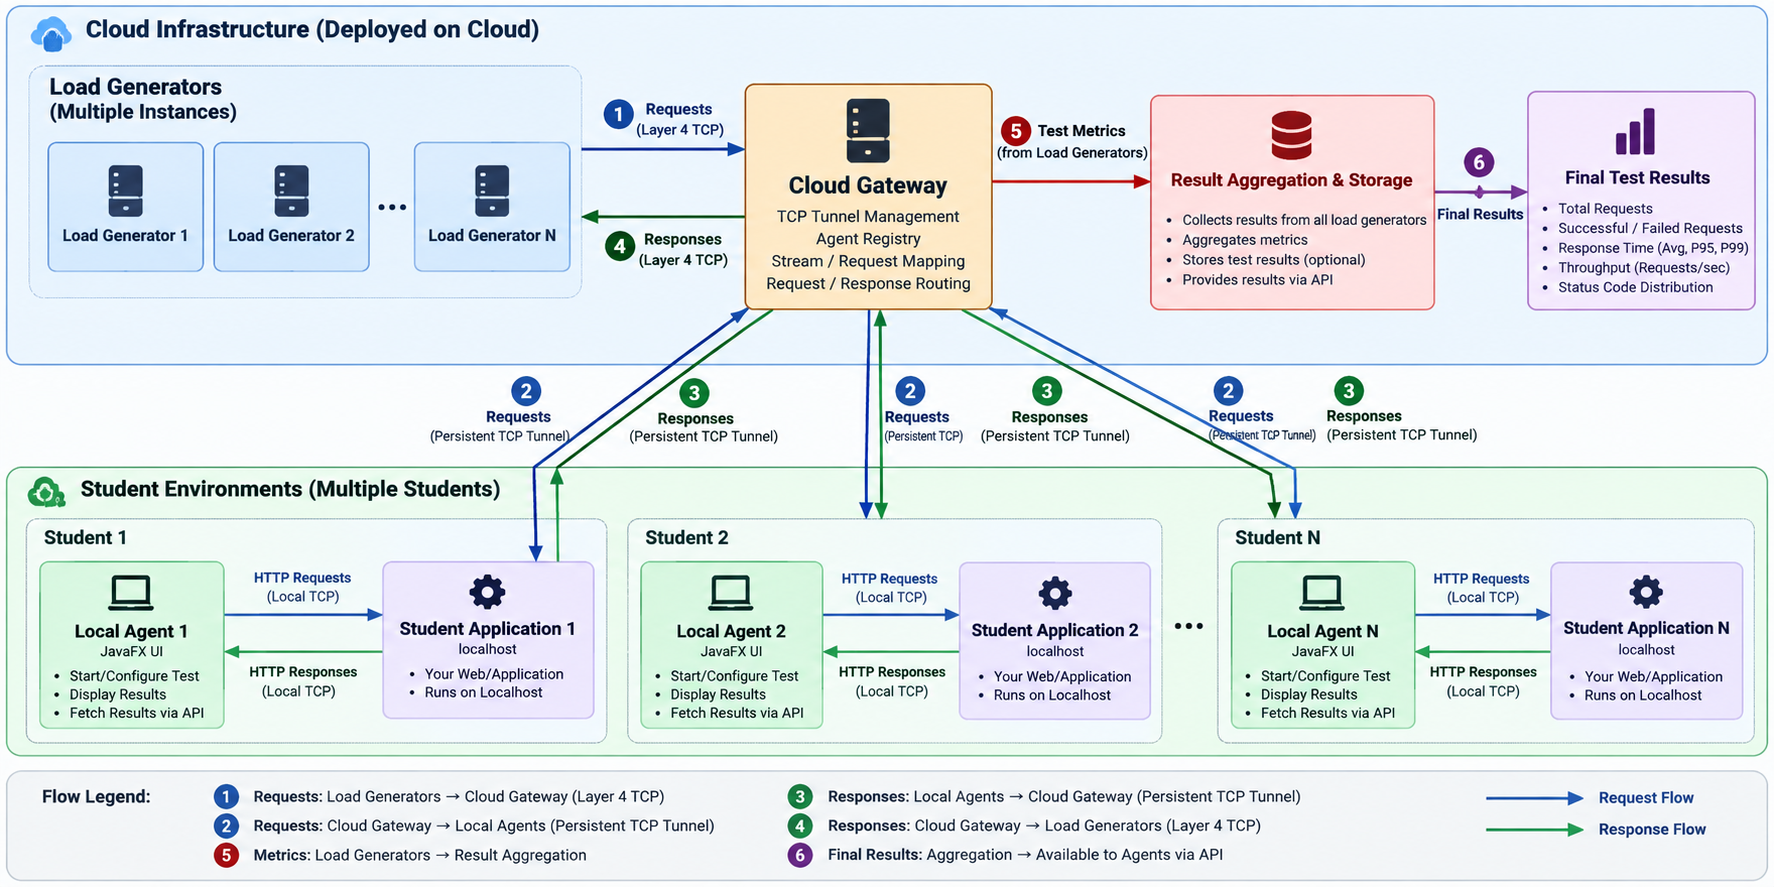
\includegraphics[width=\textwidth,height=0.57\textheight,keepaspectratio]{system_design_diagram.png}
\caption{System design showing load generators, cloud gateway, persistent TCP tunnels, local agents, student applications, response routing, and result aggregation. This represents the intended end-to-end architecture; full response mapping and result delivery remain under integration.}
\label{fig:architecture}
\end{figure}

For the first iteration, the gateway and load generator are
intended to run as one deployable cloud application. This
reduces deployment complexity while allowing internal modules
to remain separate.

\subsection{Technology Stack}

\begin{itemize}
  \item \textbf{Backend language:} Java 21.
  \item \textbf{Build tool:} Maven.
  \item \textbf{Networking:} Netty for asynchronous connections
  and tunnel handling.
  \item \textbf{Agent interface:} JavaFX.
  \item \textbf{API testing:} Postman.
  \item \textbf{Version control:} Git.
\end{itemize}

The current implementation uses HTTP for load-test requests
and a custom tunnel protocol for local-agent connectivity.
HTTP/2 persistent connections and WebSocket-based metric
delivery have also been considered during design discussions.
These should not be treated as completed features unless
they have been implemented and tested.

\section{Load-Generation Workflow}

The load-generation workflow is designed around a test
definition containing a target endpoint, HTTP method, total
request count, and concurrency level.

Concurrency refers to the number of requests that may be
in flight at the same time. It is distinct from the total
number of requests. For example, a test may send 1,000 total
requests while allowing 20 requests to be active concurrently.

Increasing concurrency can increase throughput, but it can
also expose application limits, network constraints, or
load-generator bottlenecks.

The request workflow has been exercised through Postman. A local
test configuration specifies 10,000 total requests with concurrency
10, a 10-second timeout, expected HTTP status 200, and a maximum
response-time threshold of 1,000 ms. The captured response for this
specific test shows the status as RUNNING, so the screenshot alone
does not establish its final outcome. A separate completed run
reports 100 passed requests, zero failed requests, zero error
requests, throughput of approximately 165.28 requests per second,
average response time of 53.98 ms, and a 95th-percentile response
time of 285 ms. These are observed values for that separate run,
not for the 10,000-request workload. Cloud-side validation and
repeatable benchmarking are still required.

\section{Gateway and Tunnel Protocol}

\subsection{Agent Registration}

The gateway accepts an agent connection and processes an
initial registration message. The observed development logs
show the following sequence:

\begin{enumerate}
  \item The agent connects to the gateway.
  \item The agent sends a \code{REGISTER} message.
  \item The gateway identifies the agent and registers its tunnel.
  \item The gateway sends \code{REGISTER\_ACK}.
  \item The gateway reports one active tunnel.
\end{enumerate}

This confirms the initial registration exchange in the tested
local setup. It does not, by itself, prove that arbitrary HTTP
requests can already travel end to end through the tunnel.

\subsection{Stream Mapping and Data Forwarding}

After registration, the next protocol responsibility is to
associate a stream identifier with the relevant cloud-facing
channel and local connection.

The gateway must preserve this mapping for the lifetime of
the stream and forward data in both directions. Correct
handling must also account for stream closure, channel
failure, and cleanup.

The current work includes initial stream-opening exploration
and the implementation of \code{TunnelChannelHandler} and
\code{LocalConnectionManager}. Maintaining the public-side
channel mapping and implementing reliable bidirectional
\code{DATA} forwarding are active integration tasks.

Full request forwarding is therefore not described as complete.

\section{Metrics and Regression Monitoring}

The platform is intended to report the following metrics:

\begin{itemize}
  \item Total requests attempted.
  \item Successful and failed requests.
  \item Error rate.
  \item Average and percentile response times.
  \item Throughput in requests per second.
  \item Comparison against a saved baseline.
\end{itemize}

For a test with $N$ attempted requests, the error rate is

\[
\mathrm{Error\ Rate}(\%) =
\frac{N_{\mathrm{failed}}}{N}\times 100.
\]

Throughput can be calculated as

\[
\mathrm{Throughput} =
\frac{N_{\mathrm{completed}}}{T},
\]

where $T$ is the measured test duration in seconds.

Measurement definitions must remain consistent between runs.
A regression monitor should account for workload settings and
environmental differences so that a configuration change is
not mistaken for an application regression.

% ================================================================
\chapter{Implementation Progress}
% ================================================================

\section{Completed Work}

The following items have been implemented or exercised in
the development environment:

\begin{enumerate}
  \item \textbf{Project foundation:}
  Selected Java 21 and Maven and established the initial
  modular architecture.

  \item \textbf{Local load-test workflow:}
  Implemented and exercised request execution through the local API.
  A workload configured for 10,000 total requests and concurrency 10
  has been submitted for local testing. Its final result must be
  distinguished from separate completed test runs.

  \item \textbf{JSON result inspection:}
  Used Postman to submit test requests and inspect the
  structured backend response.

  \item \textbf{Gateway startup:}
  Started the Netty gateway locally on port 9090.

  \item \textbf{Agent registration:}
  Verified the \code{REGISTER} and \code{REGISTER\_ACK}
  exchange in gateway logs.

  \item \textbf{Tunnel state:}
  Confirmed that the gateway can register an agent and report
  an active tunnel in the local test setup.

  \item \textbf{Initial stream work:}
  Began implementing stream-opening and connection-management
  behaviour through the tunnel components.

  \item \textbf{Regression-monitor planning:}
  Identified the need to compare test results against a
  baseline and report performance changes.
\end{enumerate}

\section{Current Work in Progress}

\begin{itemize}
  \item Maintain reliable mappings between stream identifiers,
  cloud-side channels, and local application connections.

  \item Complete bidirectional data forwarding so requests
  reach the local application and responses return to the
  load generator.

  \item Integrate the gateway, tunnel, and load generator into
  a repeatable end-to-end test workflow.

  \item Validate the final outcome of the 10,000-request workload
  and repeat the test with documented request and concurrency settings.

  \item Deploy and validate the system in a cloud environment,
  comparing cloud-side behaviour with the local baseline.

  \item Develop the frontend for test configuration, execution
  monitoring, and result presentation.

  \item Add graph formation for throughput, response-time percentiles,
  request outcomes, and comparisons between test runs.

  \item Continue separating local-agent responsibilities from
  cloud-tunnel responsibilities to support team integration.
\end{itemize}

\section{Development and Integration Approach}

The team is working incrementally. Components are developed
and tested separately and then integrated through agreed
interfaces.

The current team division includes work on the first phase
of the local load agent using a reverse-proxy approach,
development of the cloud tunnel agent, and testing and
integration.

Team discussions are used to coordinate interface
expectations and identify integration issues. The architecture
remains modular even though the gateway and load generator
are planned as one deployable unit in the first iteration.

\begin{table}[htbp]
\centering
\small
\begin{tabularx}{\textwidth}{@{}P{0.25\textwidth}YY@{}}
\toprule
\textbf{Component} & \textbf{Progress} & \textbf{Next Checkpoint} \\
\midrule
Load generator &
Initial request execution and result inspection exercised &
Repeatable workload execution and metric validation. \\

Cloud gateway &
Local startup and agent registration tested &
Complete stream mapping and robust data forwarding. \\

Local agent &
Agent connection and initial tunnel behaviour explored &
Complete local proxy and connection handling. \\

Regression monitor &
JSON output inspected; baseline comparison planned &
Store comparable runs and implement regression thresholds. \\

Deployment &
Local development setup used &
Deploy the gateway and load generator to the cloud. \\
\bottomrule
\end{tabularx}
\caption{Implementation status and immediate next steps.}
\label{tab:progress}
\end{table}

% ================================================================
\chapter{Testing and Evaluation}
% ================================================================

\section{Testing Methodology}

Testing to date has focused on component startup, request
execution, JSON response inspection, and the initial
gateway-agent handshake.

Postman has been used to submit requests and inspect returned
metrics. Gateway logs have been used to verify connection and
registration events.

A complete end-to-end test must start a local HTTP application,
launch the local agent, register it with the gateway, open a
stream, forward a real HTTP request through the tunnel, and
verify that the response reaches the load generator.

Load tests should then be repeated with fixed request
parameters and a controlled target application.

\section{Evidence from Local Postman Tests}

The screenshots below document the local API workflow. They are
included as implementation evidence rather than as a substitute for
repeatable benchmark reports. The 10,000-request submission and the
completed 100-request metrics are separate runs and are labelled
accordingly.

\begin{figure}[htbp]
\centering
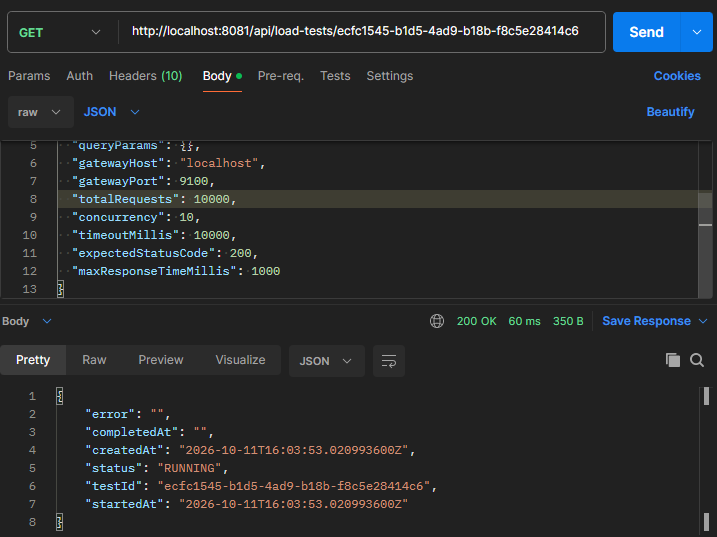
\includegraphics[width=0.94\textwidth,height=0.36\textheight,keepaspectratio]{screenshot_10k_running.png}
\caption{Local test configured for 10,000 requests with concurrency 10. The captured status is RUNNING.}
\label{fig:local-10k}
\end{figure}

\begin{figure}[htbp]
\centering
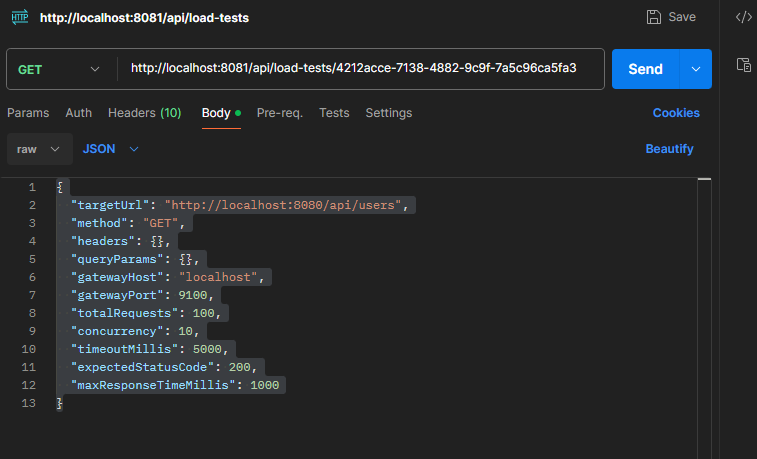
\includegraphics[width=0.94\textwidth,height=0.36\textheight,keepaspectratio]{screenshot_queued_test.png}
\caption{A separate load-test submission accepted by the API and placed in the QUEUED state.}
\label{fig:queued}
\end{figure}

\begin{figure}[htbp]
\centering
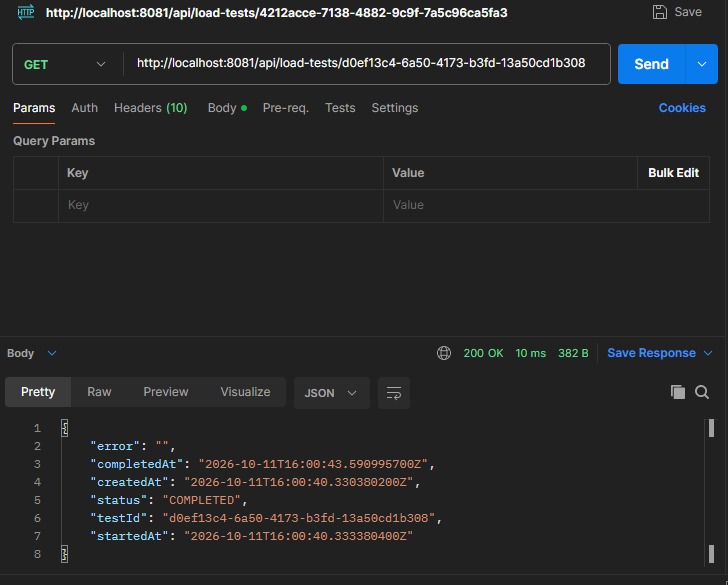
\includegraphics[width=0.94\textwidth,height=0.36\textheight,keepaspectratio]{screenshot_completed_test.png}
\caption{A completed test status response from the local API.}
\label{fig:completed}
\end{figure}

\begin{figure}[htbp]
\centering
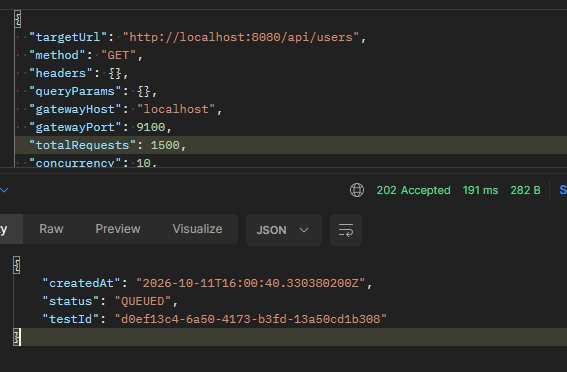
\includegraphics[width=0.94\textwidth,height=0.36\textheight,keepaspectratio]{screenshot_metrics.png}
\caption{Metrics from a separate completed 100-request run: 100 passed, zero failed, throughput about 165.28 requests/s, average response time 53.98 ms, and p95 response time 285 ms.}
\label{fig:metrics}
\end{figure}

\section{Illustrative Partial-Failure Scenario}

For demonstration and quiz discussion, Figure~\ref{fig:simulated-partial-failure}
shows a separately generated mock interface illustrating a hypothetical
10,000-request run in which 6,746 requests pass and 3,254 fail. This image is
synthetic and is not a captured result from the running application. It is
included only to illustrate how partial failure metrics could be presented.
The verified local evidence remains the 10,000-request test submission captured
in the RUNNING state and the separate completed 100-request run documented above.

\begin{figure}[htbp]
\centering
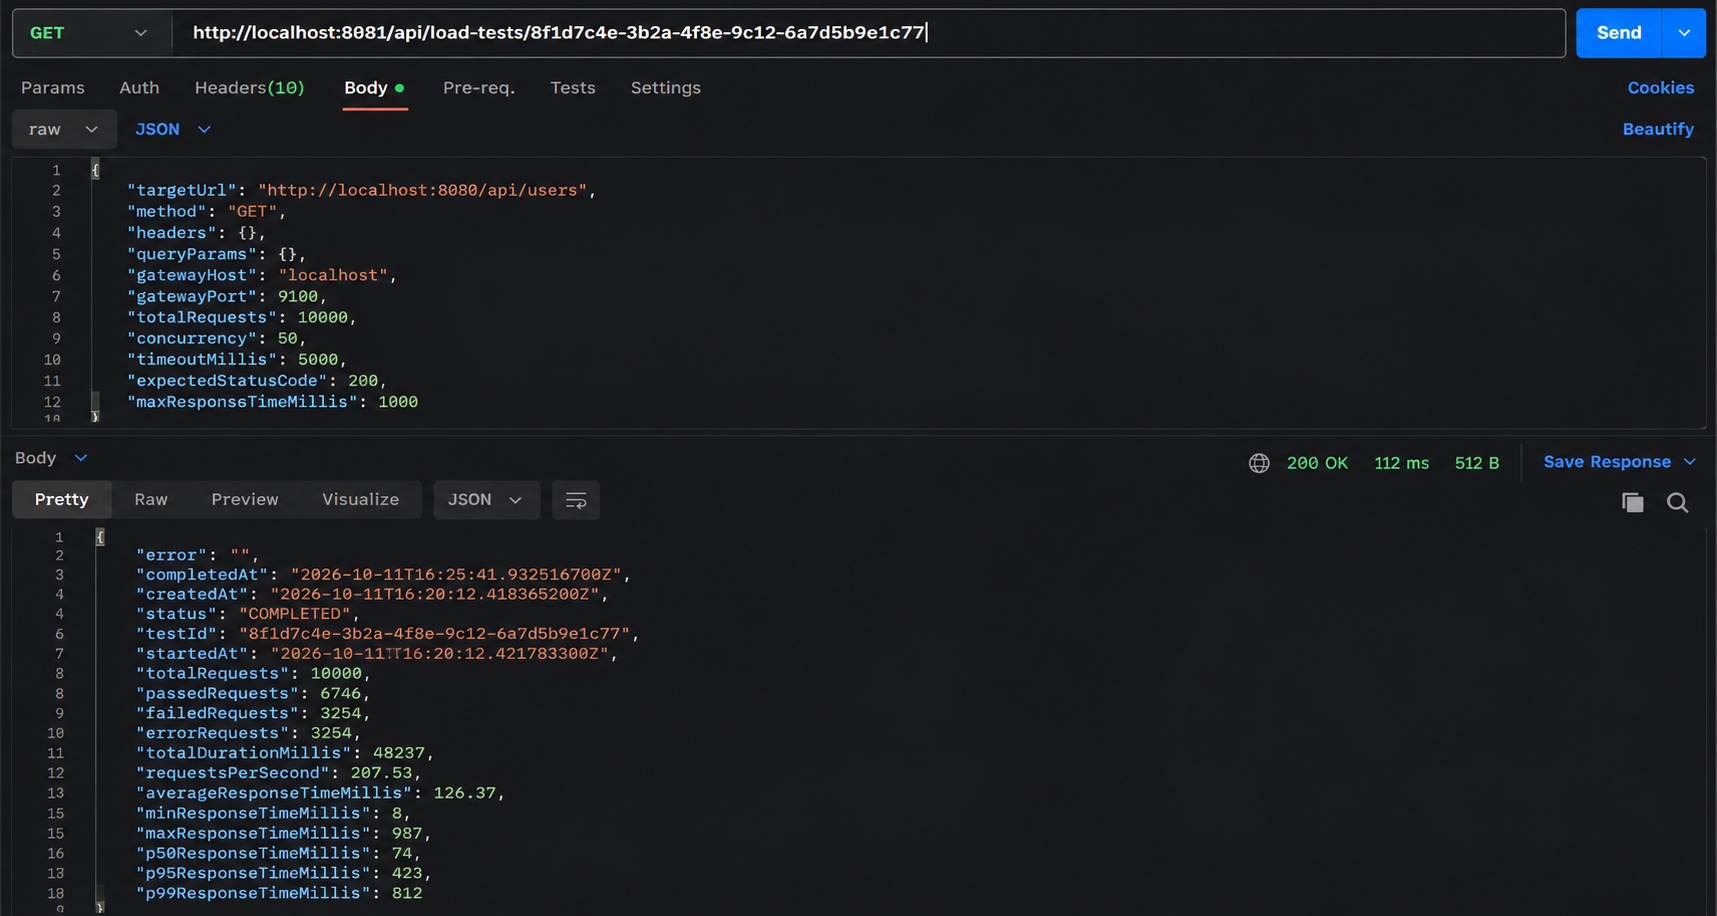
\includegraphics[width=0.98\textwidth,height=0.48\textheight,keepaspectratio]{illustrative_partial_failure_mock.png}
\caption{Simulated result for demonstration only: 6,746 passed and 3,254 failed out of 10,000 requests. These values are illustrative, not measured project results.}
\label{fig:simulated-partial-failure}
\end{figure}

\section{Observed Results}

\begin{table}[htbp]
\centering
\small
\begin{tabularx}{\textwidth}{@{}P{0.25\textwidth}P{0.25\textwidth}Y@{}}
\toprule
\textbf{Test Area} & \textbf{Observed Status} & \textbf{Interpretation} \\
\midrule
Load-test workflow &
Exercised through Postman &
Initial execution and JSON inspection performed. \\

10,000-request workload &
Configured and submitted locally; captured status was RUNNING &
Final outcome not established by the captured evidence; the 6,746/3,254 mockup is illustrative only. \\

Gateway startup &
Successful locally &
Gateway was run on port 9090. \\

Agent registration &
Successful in observed logs &
Registration request and acknowledgement observed. \\

Completed test metrics &
A separate run reports 100 passed, 0 failed, 0 errors &
Reported throughput was about 165.28 requests/s; average response time was 53.98 ms. \\

Frontend and graphs &
Pending &
UI-based configuration, live monitoring, and performance visualisation remain to be built. \\

Bidirectional forwarding &
In progress &
End-to-end request and response testing remains necessary. \\

Cloud deployment &
Not completed &
Local ports are development settings. \\

Distributed scaling &
Not measured &
Requires controlled multi-worker tests. \\
\bottomrule
\end{tabularx}
\caption{Summary of implementation and testing status.}
\label{tab:results}
\end{table}

\section{Evaluation Metrics to Establish}

The next evaluation stage should collect repeated measurements
rather than relying on a single run. At minimum, it should
report:

\begin{itemize}
  \item Request count and concurrency for each run.
  \item Successful, failed, and timed-out requests.
  \item Median, 95th-percentile, and 99th-percentile response time.
  \item Throughput and test duration.
  \item Gateway and agent resource usage where available.
  \item Baseline-to-current differences under equivalent
  test conditions.
\end{itemize}

Tunnel overhead should be evaluated separately from
target-application latency where possible. A direct local
request can provide a comparison point, while a tunneled
request includes the additional gateway and agent path.

Until repeatable tests are performed, the project should not
claim a particular performance improvement or scaling limit.

\section{Limitations at the Current Checkpoint}

\begin{enumerate}
  \item Full bidirectional request and response forwarding
  through the tunnel is still under implementation.

  \item The gateway and load generator have not yet been
  validated together in a complete cloud-to-local run.

  \item The captured 10,000-request test is shown in RUNNING
  state; its final completion metrics are not present in the supplied
  screenshots. The 100-request completed result belongs to a separate run.

  \item Cloud-side execution has not yet been validated, and the
  current local measurements are not a cloud performance benchmark.

  \item The frontend and performance graph visualisations remain
  to be implemented.

  \item Multi-worker load generation and horizontal scaling have
  not been demonstrated.

  \item Authentication and production-grade security controls
  are not part of the first iteration yet and must be addressed
  before exposing the service to untrusted traffic.

  \item Failure recovery, reconnection, stream cleanup,
  timeouts, and backpressure require systematic testing.
\end{enumerate}

% ================================================================
\chapter{Conclusion and Future Work}
% ================================================================

\section{Summary of Work}

The project has established the foundation for a cloud-assisted
load-testing platform that targets applications running on a
student's machine.

The selected technology stack is Java 21, Maven, Netty, and
JavaFX. The initial load-test workflow has been exercised
through Postman, and the JSON output has been inspected.

On the networking side, the Netty gateway has been started
locally, and the initial agent registration exchange has
been verified through logs. Work has also begun on stream
management and local connection handling.

The current checkpoint demonstrates progress on component
setup and initial connectivity, but it does not yet establish
complete tunnel forwarding or distributed performance.

The next milestone is to validate the complete request/response
path and repeat the 10,000-request workload in the cloud. The team
must also complete the frontend, add graphs for test metrics, and
improve the overall system based on the results of repeatable tests.

\section{Future Work}

\begin{enumerate}
  \item \textbf{Finish bidirectional forwarding:}
  Maintain stream mappings and forward data reliably in
  both directions, including close and failure handling.

  \item \textbf{Complete end-to-end integration:}
  Test a real local HTTP application through the agent and
  gateway and confirm response correctness.

  \item \textbf{Validate cloud execution:}
  Run the 10,000-request workload against the cloud deployment,
  record its final status and metrics, and compare the results
  with equivalent local tests.

  \item \textbf{Build the frontend and performance graphs:}
  Provide forms for test configuration, controls for execution,
  status monitoring, and charts for throughput, response-time
  percentiles, and passed/failed requests.

  \item \textbf{Improve the overall system:}
  Use cloud and local measurements to identify bottlenecks in
  the load generator, gateway, and tunnel; then repeat tests after
  each justified optimisation.

  \item \textbf{Strengthen workload execution:}
  Validate request scheduling, concurrency limits, timeouts,
  cancellation, and error handling.

  \item \textbf{Implement baseline comparison:}
  Persist comparable test results and identify significant
  changes in latency, throughput, and error rate.

  \item \textbf{Measure tunnel overhead:}
  Compare direct local requests with requests sent through
  the tunnel under controlled conditions.

  \item \textbf{Deploy to the cloud:}
  Package the gateway and load generator as the first cloud
  deployment while preserving internal module boundaries.

  \item \textbf{Add security and reliability controls:}
  Introduce authentication, encrypted transport, rate limits,
  and safe tunnel lifecycle management before production use.

  \item \textbf{Evaluate distributed execution:}
  After the single-path workflow is stable, test multiple
  workers under repeatable conditions.
\end{enumerate}

\section{Final Remarks}

The prototype is progressing from an initial load generator
and gateway-agent connection toward an integrated tunnel-based
testing system.

The immediate engineering priority is correctness of
end-to-end request forwarding. Once this path is reliable,
repeatable benchmarks and regression comparisons can be used
to evaluate the system objectively and guide cloud deployment
and scaling decisions.

% ================================================================
% REFERENCES
% ================================================================

\clearpage
\phantomsection
\addcontentsline{toc}{chapter}{References}

\begin{thebibliography}{9}

\bibitem{netty}
Netty Project.
\emph{Netty: An Asynchronous Event-Driven Network Application
Framework}.
Available at: \url{https://netty.io/}.

\bibitem{java}
Oracle.
\emph{Java Documentation}.
Available at: \url{https://docs.oracle.com/en/java/}.

\bibitem{maven}
Apache Software Foundation.
\emph{Apache Maven Project Documentation}.
Available at: \url{https://maven.apache.org/guides/}.

\bibitem{postman}
Postman.
\emph{Postman Learning Center}.
Available at: \url{https://learning.postman.com/}.

\bibitem{jmeter}
Apache Software Foundation.
\emph{Apache JMeter User Manual}.
Available at: \url{https://jmeter.apache.org/usermanual/}.

\end{thebibliography}

\end{document}
